\documentclass{article}
\usepackage{graphicx} % Required for inserting images
\usepackage[italian]{babel}
\usepackage{amsmath}
\usepackage[hidelinks]{hyperref}
\usepackage{float}
\usepackage{multicol}
\usepackage{changepage}

\title{Architettura degli elaboratori}
\author{Leonardo Ganzaroli}
\date{}

\begin{document}

\maketitle

\addcontentsline{toc}{section}{\protect\numberline{}Introduzione}

\tableofcontents

\hypersetup{allcolors=black}

\newpage

\section*{Introduzione}

Questi appunti sono derivanti principalmente dalle slide del corso di \textit{Architettura degli elaboratori} che ho svolto durante la laurea Triennale di informatica all'università "La Sapienza".\newline

\noindent \textbf{N.B. Questo corso è il naturale proseguimento di \textit{Progettazione di Sistemi Digitali}, quindi molte cose saranno date per scontate}.

\newpage

\section{Argomenti introduttivi}

\subsection{Cenni storici}

\textbf{Definizione} L'alfabeto numerico è un insieme di simboli atti a rappresentare quantità di beni.\newline

\noindent I metodi per rappresentare quantità ed effettuare calcoli su di esse esistono da migliaia di anni e nel corso del tempo si sono evoluti fino a diventare automatici: 
\begin{itemize}
    
    \item \textbf{Manuale} 
        \begin{itemize}
            \item \textbf{Osso di Lebombo} (circa 35000 a.c.)

                Uno dei più antichi manufatti mai ritrovati ad uso matematico.
            
            \item \textbf{Tavoletta d'argilla} 

            \item \textbf{Abaco} 

            \item \textbf{Macchina di Anticitera} (100-150 a.c.)

                Planetario meccanico usato per calcolare le fasi lunari, il movimento dei pianeti, etc$\ldots$

            \item \textbf{Sistema decimale posizionale} (1202)\newline
            
        \end{itemize}

    \item \textbf{Semi-manuale}
        \begin{itemize}
            \item \textbf{Calculating Clock} (1623)

                La prima calcolatrice meccanica.

            \item \textbf{Pascalina} (1642)

                Macchina che consente di svolgere addizioni e sottrazioni.

            \item \textbf{Contatore a gradini} (1672)

                Evoluzione della Pascalina che permette di svolgere anche moltiplicazioni e divisioni.

            \item \textbf{Aritmometro} (1727)

                Miglioramento del contatore a gradini.

            \item \textbf{Macchina differenziale} (1816)

                Macchina a vapore che permetteva di svolgere anche il calcolo polinomiale.\newline
            
        \end{itemize}

    \item \textbf{Macchine programmabili}
        \begin{itemize}

            \item \textbf{Macaroni Box} (1889)

                Prima calcolatrice con tastiera che riproduceva il risultato su nastro cartaceo.
        
            \item \textbf{Tabulator Machine} (1890)

                Primo prototipo di macchina automatica per il censimento, usava schede cartacee perforabili.

            \item \textbf{Macchina di Turing} (1935)

            \item \textbf{Atanasoff Berry Computer} (1942)

                Primo calcolatore totalmente elettronico.

            \item \textbf{Colossus} (1944)

                Primo calcolatore digitale. 

            \item \textbf{Mark III} (1950)

                Primo uso di un nastro magnetico come memoria di massa.

            \item \textbf{UNIVersal} (1951)

                Elaboratore ad uso generico, programmi redatti tramite lo \textit{Short Order Code}.

            \item \textbf{RAMAC} (1957)

                Primo uso di un Hard-disk come memoria di massa.

            \item \textbf{CEP} (1961)

                Il primo calcolatore elettronico italiano usato per le ricerche scientifiche.\newline
            
        \end{itemize}

        \item \textbf{Minicomputer}

            A partire dagli anni sessanta ci fu una nuova generazione di calcolatori con costo e stazza ridotti:
            \begin{itemize}
                \item \textbf{PDP-1} (1960)
                \item \textbf{Xerox Alto} (1970)

                    Aveva un sistema operativo con una rudimentale interfaccia grafica.\newline
                    
            \end{itemize}

        \item \textbf{Microcomputer}

            Un decennio dopo ci fu la nascita dei microprocessori, i più importanti sono:
            \begin{itemize}
                \item \textbf{Intel 4004} (1971)
                \item \textbf{Intel 8008} (1972)

                    Primo uso di un registro apposito per gli indirizzi.

                \item \textbf{Intel 8085} (1976)

                    Sfruttava il DMA e le interruzioni vettorizzate che portarono ad un miglioramento delle comunicazioni I/O e del multitasking.

                \item \textbf{Intel 8086} (1978)

                    Aveva una gestione segmentata della memoria, ciò permetteva la rilocazione dei programmi.

                \item \textbf{Motorola 68000} (1979)

                    Utilizzava un multi-bus per trasferire informazioni eterogenee.

                \item \textbf{Intel 80286} (1982)

                    Primo uso della memoria virtuale.\newline
                
            \end{itemize}

        \item \textbf{Seconda generazione}
            \begin{itemize}
                \item \textbf{MIPS} (1982)

                    Grazie all'uso della \textit{pipeline} aveva delle ottime prestazioni.

                \item Nel 1984 Sony e Philips presentano il \textbf{CD-ROM}

                \item \textbf{Intel 80386} (1985)

                    Primo uso del cahing della memoria.

                \item \textbf{ARM2} (1987)

                    Processore dotato di un coprocessore matematico.

                \item \textbf{Intel 80486} (1989)

                    Primo uso del \textit{Read-Ahead}.\newline
                
            \end{itemize}
            
        \item \textbf{Terza generazione}
            \begin{itemize}
                \item \textbf{Pentium} (1993)
                \item \textbf{Pentium Pro} (1995)

                    Utilizzava la Cache di 2° livello e l'esecuzione \textit{Out of Order}.

                \item \textbf{Pentium II} (1997)

                    Introduzione della tecnologia \textit{MMX} per l'elaborazione audio e video.

                \item \textbf{Pentium III} (1999)

                    Conteneva l'estensione \textit{SSE} che portò ad un potenziamento del coprocessore matematico.\newline
                
            \end{itemize}

        \item A partire dal 2001 si iniziò a puntare sul parallelismo tramite processori multipli e multicore:
        \begin{itemize}
            \item \textbf{Pentium D} (2005)

                Dotato di 2 core e cache condivisa tra essi.

            \item \textbf{Intel i3,i5,i7,i9} (2010-\ldots)

                Tre livelli di Cache e uso dell'\textit{HyperMultiThreading}.\newline
            
        \end{itemize}

\end{itemize}

\subsection{Richiami di teoria dell'informazione}

La teoria pone l'attenzione sul come inviare un messaggio (concatenazione di simboli/segnali/parole) e ricostruirlo poi in modo esatto, inoltre propone uno schema generale di un sistema di comunicazione:
\begin{enumerate}
    \item \textbf{Sorgente} = insieme delle possibili parole
    \item \textbf{Trasmettitore} = entità che codifica una parola in un segnale
    \item \textbf{Canale} = mezzo con cui si propaga il segnale
    \item \textbf{Ricevente} = intermediario che decodifica il segnale
    \item \textbf{Ricevente} 
\end{enumerate}

\begin{figure}[ht]
    \centering
    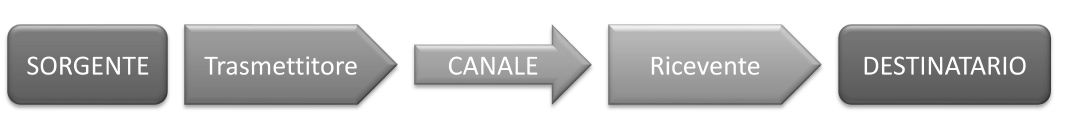
\includegraphics[width=\linewidth]{comm.png}
    \caption{Schema generale}
    \label{fig:comm}
\end{figure}

\newpage

\section{Macchina di Von Neumann}

\textbf{Definizione} La macchina di Von Neumann è un modello generale di elaboratore che prevede l'archiviazione di dati e istruzioni nella stessa memoria e la possibilità di effettuare salti nel programma.
\begin{figure}[ht]
    \centering
    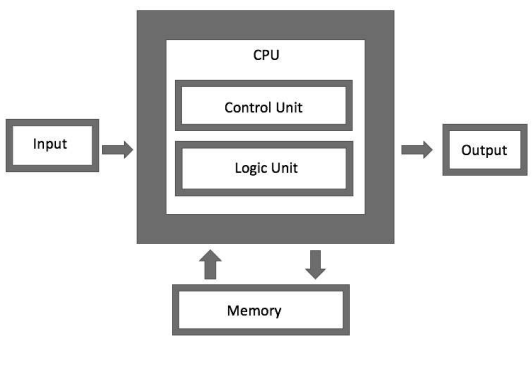
\includegraphics[width=\linewidth]{von_neumann.png}
    \caption{Modello di Von Neumann}
    \label{fig:von_neumann}
\end{figure}

\newpage

\subsection{Componenti}

\begin{itemize}
    \item \textbf{CU}

    La Control Unit è predisposta a scandire le operazioni elementari necessarie per eseguire ogni istruzione.

\begin{figure}[ht]
    \centering
    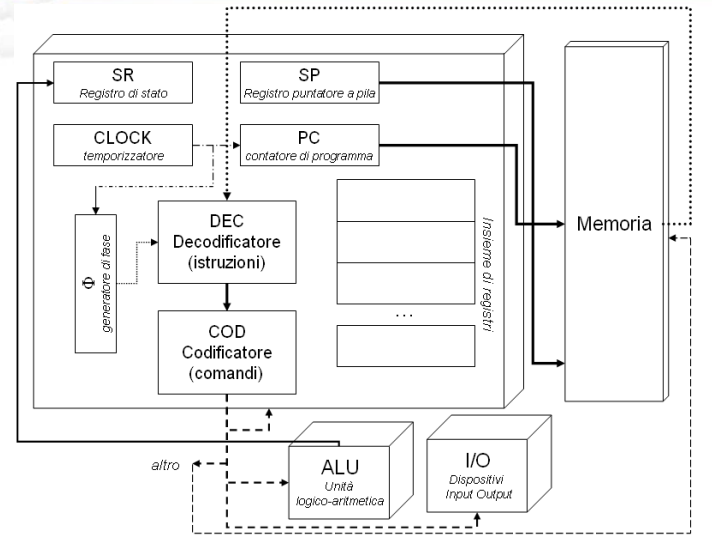
\includegraphics[width=\linewidth]{vonn_comp.png}
    \caption{Control Unit}
    \label{fig:von_comp}
\end{figure}

        \begin{itemize}
            \item I \textbf{registri} sono delle piccole memorie presenti internamente alla CU, sono di 2 tipi:
            \begin{itemize}
                \item Ad uso \textbf{speciale}:
                    \begin{itemize}
                        \item \textbf{Program Counter}

                            Contiene l'indirizzo dell'istruzione da seguire attualmente.

                        \item \textbf{Status Register}

                            Contiene informazioni riguardo lo stato della CU.

                        \item \textbf{Stack Pointer}

                            Contiene l'indirizzo della cima della pila.
                        
                    \end{itemize}

                    \item Ad uso \textbf{generale}

                        Usati per mantenere risultati di operazioni e/o informazioni di controllo.
                    
            \end{itemize}

            \newpage

            \item \textbf{Generatore di fase}

                Scandisce le varie di fasi di esecuzione delle operazioni elementari, quest'ultime si possono riassumere in:
                \begin{enumerate}
                    \item \textbf{Caricamento}

                        Lettura dell'indirizzo nel PC.
                        
                    \item \textbf{Decodifica}

                        Riconoscimento di operazione ed operandi.
                    
                    \item \textbf{Esecuzione}
                    
                    \item \textbf{Spostamento}\newline
                \end{enumerate}

                Ogni istruzione ha bisogno di un certo numero di cicli macchina per essere eseguita, questi possono essere diversi e dipendono da molti fattori.\newline

        \item \textbf{Transcodificatore}

            Riconosce le istruzioni e genera gli opportuni comandi.\newline

        \end{itemize}

    \item \textbf{ALU}

        L'unità logico-aritmetica si occupa di effettuare operazioni logiche 
        ed aritmetiche.

\begin{figure}[ht]
\centering
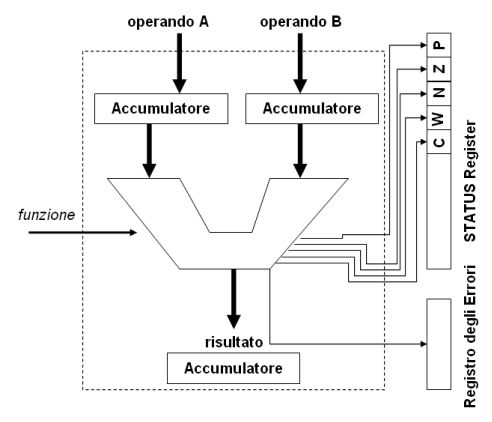
\includegraphics[width=0.8\linewidth]{ALU.png}
\caption{ALU}
\label{fig:alu}
\end{figure}

    \begin{itemize}
        \item \textbf{Accumulatori}

            Sono dei registri "trasparenti" che ospitano gli operandi/soluzioni durante le operazioni.

        \item \textbf{Registro degli errori}

            Usato per indicare situazioni non risolvibili.

        \item \textbf{Funzione}

            Un input che indica l'operazione da eseguire.

        \item \textbf{Flags}

            Output che forniscono informazioni sul'ultima operazione eseguita.\newline
        
    \end{itemize}

    \item \textbf{Memoria}

        Ha delle aree riservate contenenti informazioni essenziali per il funzionamento e per operazioni particolari. Nel caso di memorie con dimensioni importanti si ricorre ad una divisione logica per semplificare l'accesso, essa viene divisa in banchi e blocchi e l'indirizzo viene sezionato.\newline

        \begin{figure}[ht]
            \centering
            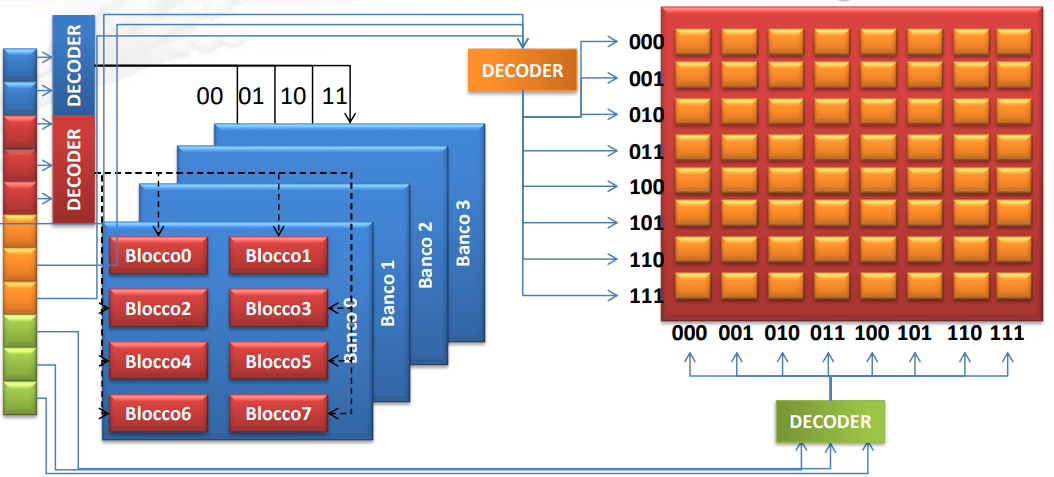
\includegraphics[width=\linewidth]{ram.png}
            \caption{4 banchi, 8 blocchi}
            \label{fig:ram}
        \end{figure}

    \item \textbf{Dispositivi I/O}

        Permettono di collegare l'elaboratore con il mondo esterno in diversi modi, un problema di questa interazione è il fatto che i dispositivi hanno delle velocità di trasferimento delle informazioni estremamente minore rispetto alle componenti interne e ciò porta problemi di sincronizzazione.\newline

        \newpage

        Visto il possibile trasferimento di dati è opportuno usare un protocollo per regolarlo:
        
\begin{figure}[ht]
    \begin{minipage}[t]{0.49\textwidth}
        \centering
        \begin{figure}[H]
        \centering
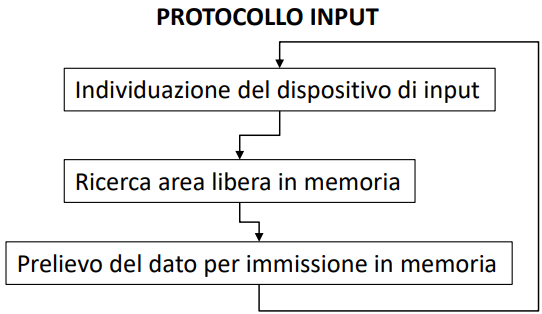
\includegraphics[width=.7\linewidth]{prot_in.png}
        \end{figure}
        \label{fig:p_in}
    \end{minipage}
    \begin{minipage}[t]{0.49\textwidth}
        \centering
        \begin{figure}[H]
        \centering
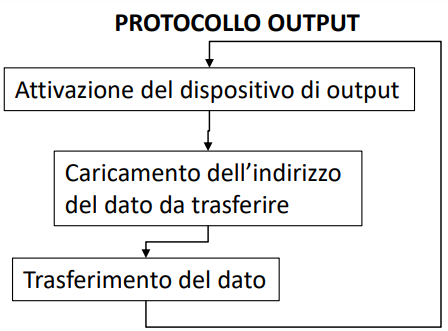
\includegraphics[width=.65\linewidth]{prot_out.png}
        \end{figure}
        \label{fig:p_out}
    \end{minipage}
\end{figure}

    In ogni caso un dispositivo va interconnesso ad un modulo I/O, esso fa da intermediario con il processore:

    \begin{itemize}
        \item \textbf{INPUT}

        \begin{figure}[ht]
        \centering
        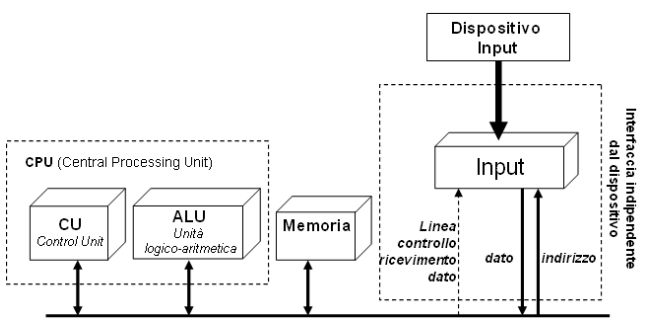
\includegraphics[width=0.71\linewidth]{in.png}
        \label{fig:in_contr}
        \end{figure}

        \begin{figure}[ht]
        \centering
        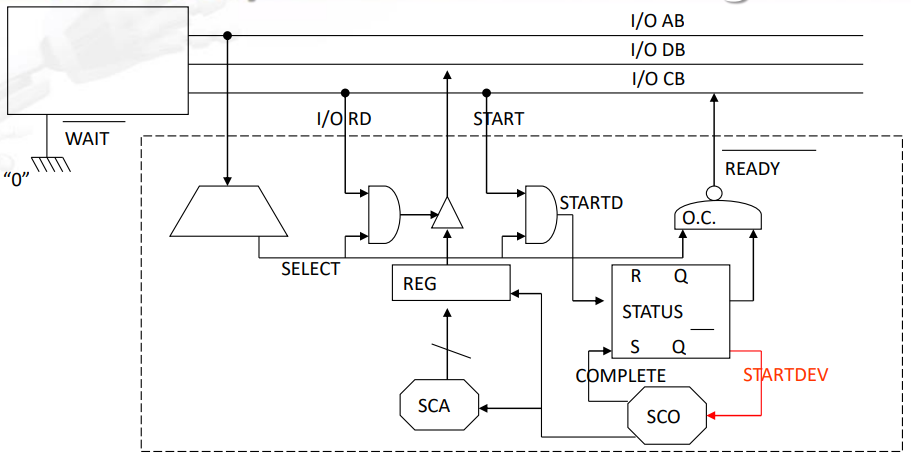
\includegraphics[width=0.71\linewidth]{in2.png}
        \label{fig:in_contr2}
        \caption{Controller Input dettagliato}
        \end{figure}

        \newpage

        Protocollo:
        \begin{enumerate}
            \item il processore invia sull’I/O Address bus l’indirizzo del dispositivo e ne esamina lo stato tramite la linea di controllo $\overline{\text{READY}}$

            \item Se il dispositivo non è pronto il processore deve attendere e tornare al punto 1,  se è pronto va al punto 3

            \item START resetta il flip-flop STATUS e in tale stato rimane per tutta la durata delle operazioni

            \item Quando il dato è disponibile in REG, il dispositivo genera il segnale COMPLETE, settando STATUS

            \item Nel frattempo il processore, in attesa del dato, esamina il flip-flop STATUS campionando il segnale READY

            \item Se $\overline{\text{READY}}=1$ il processore deve attendere e tornare al punto 5, altrimenti invia il segnale di controllo IO/RD per trasferire il dato presente in REG nella locazione di memoria che ospiterà il valore \newline

        \end{enumerate}

        \item \textbf{OUTPUT}

        \begin{figure}[ht]
        \centering
        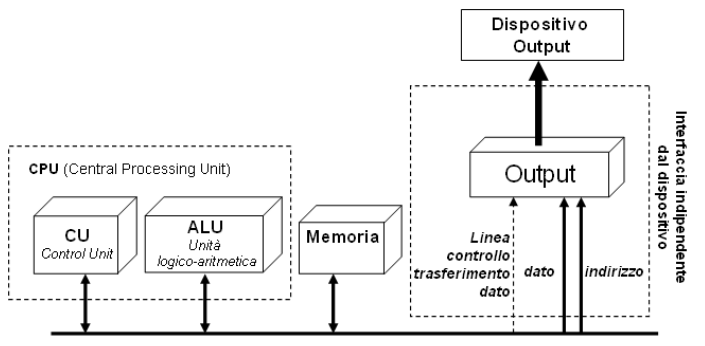
\includegraphics[width=0.71\linewidth]{out.png}
        \label{fig:out_contr}
        \end{figure}

        \begin{figure}[ht]
        \centering
        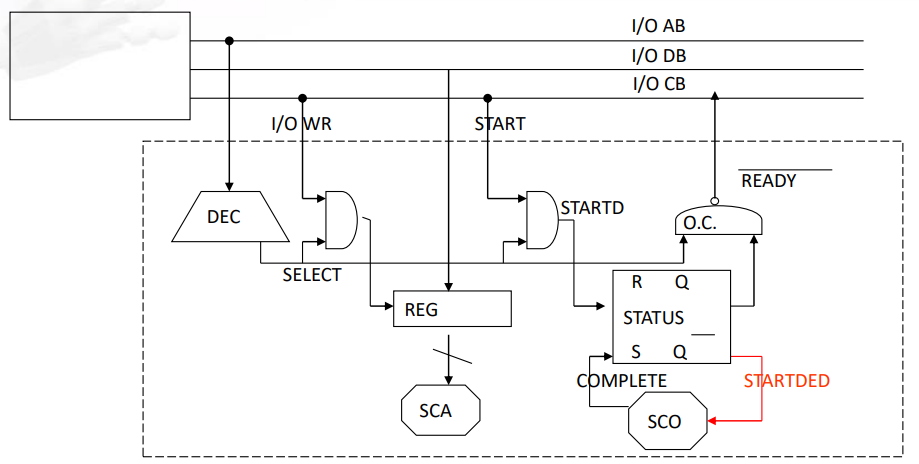
\includegraphics[width=0.71\linewidth]{out2.png}
        \label{fig:out_contr2}
        \caption{Controller Output dettagliato}
        \end{figure}

        \newpage

        Protocollo:
        \begin{enumerate}
            \item il processore invia sull’I/O Address bus l’indirizzo del dispositivo e ne esamina lo stato tramite la linea di controllo $\overline{\text{READY}}$

            \item Se il dispositivo non è pronto il processore deve attendere e tornare al punto 1,  se è pronto va al punto 3

            \item Il processore trasferisce il contenuto dalla locazione di memoria al registro d'interfaccia del dispositivo

            \item Il processore invia il segnale START che resetta il flip-flop STATUS e in tale stato rimane per tutta la durata delle operazioni, quando il dato è stato letto il dispositivo genera il segnale COMPLETE che setta STATUS

            \item Nel frattempo il processore, in attesa del dato, esamina il flip-flop STATUS campionando il segnale $\overline{\text{READY}}$

            \item Se $\text{READY}=1$ il processore deve attendere e tornare al punto 5, altrimenti può eseguire un'altra istruzione\newline

        \end{enumerate}

        Per quanto riguarda l'accesso da/ai dati e l'indirizzamento dei dispositivi si usano 2 tecniche:
            \begin{enumerate}
                \item \textbf{I/O Canonico}

                    Si riserva uno spazio indipendente con specifiche istruzioni.

                \item \textbf{I/O programmato}

                    Si riserva una parte della memoria centrale.
                
            \end{enumerate}

        \begin{figure}[ht]
        \centering
        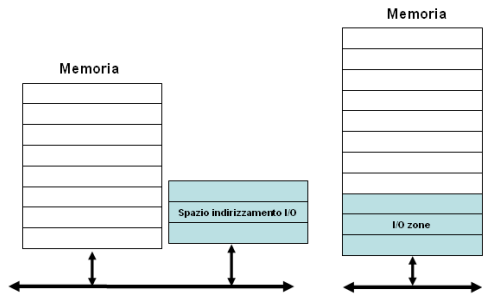
\includegraphics[width=0.8\linewidth]{io_can_prog.png}
        \label{fig:io}
        \caption{Canonico e Programmato}
        \end{figure}
        
    \end{itemize}

    \newpage

    \item \textbf{Interconnessioni}
        \begin{itemize}
            \item \textbf{Punto a punto}
        
                Si usa per effettuare trasferimenti da un registro ad un altro.

                        \begin{figure}[ht]
                        \centering
                        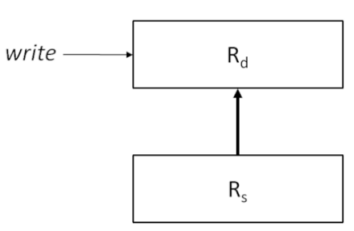
\includegraphics[width=0.4\linewidth]{p2p.png}
                        \label{fig:p2p}
                        \end{figure}

            \item \textbf{Multiplexer}

                Si usa per effettuare trasferimenti da molti registri ad uno.

                        \begin{figure}[ht]
                        \centering
                        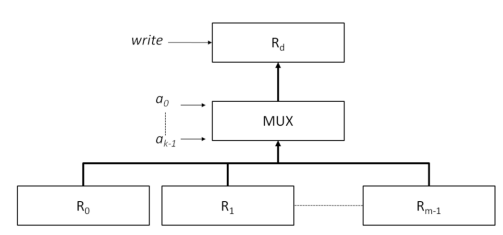
\includegraphics[width=0.7\linewidth]{mult.png}
                        \label{fig:mult}
                        \end{figure}

            \item \textbf{Demultiplexer}

                Si usa per effettuare trasferimenti da un registro a molti.

                        \begin{figure}[ht]
                        \centering
                        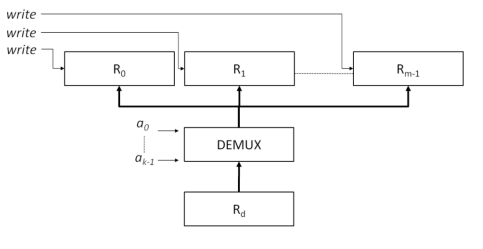
\includegraphics[width=0.7\linewidth]{demult.png}
                        \label{fig:demult}
                        \end{figure}

            \newpage

            \item \textbf{Mesh}

                Permette di connettere molti componenti tra loro.

                        \begin{figure}[ht]
                        \centering
                        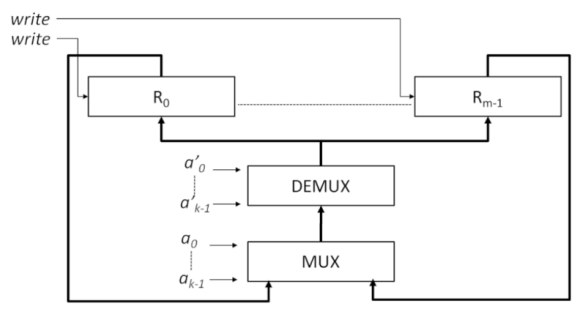
\includegraphics[width=0.7\linewidth]{mesh.png}
                        \label{fig:mesh}
                        \end{figure}

            \item \textbf{Bus}

                Fascio di $n$ linee, tramite il buffer tristate si può scegliere quale attivare.\newline

                        \begin{figure}[ht]
                        \centering
                        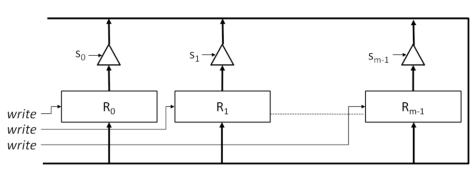
\includegraphics[width=0.7\linewidth]{bus.png}
                        \label{fig:bus}
                        \end{figure}

                Oggigiorno vengono usati bus multipli o multiplexati che permettono di averne uno tra processore e memoria ed almeno un altro per le periferiche.\newline

                \newpage

                Per risolvere il problema delle richieste simultanee si utilizza l'arbitraggio:
                \begin{itemize}
                    \item \textbf{Centralizzato}

                        Un'entità chiamata arbitro decide qual'è il prossimo dispositivo usando il \textit{daisy chaining}, è possibile usare diverse linee con diverse priorità.

                        \begin{figure}[ht]
                        \centering
                        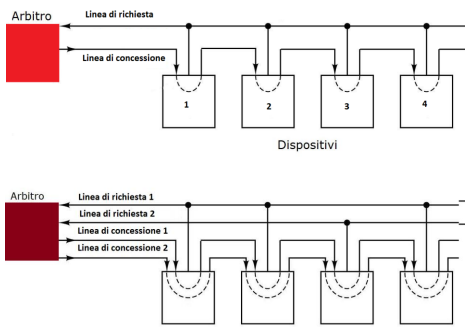
\includegraphics[width=0.7\linewidth]{arb_centr.png}
                        \label{fig:arb_centr}
                        \end{figure}                        

                    \item \textbf{Decentralizzato}

                        Si usano diverse linee con diverse priorità, quando un dispositivo deve usare il bus invia un segnale sulla linea di richiesta ed analizza le linee per sapere se è il prossimo a poterlo usare.

                        \begin{figure}[ht]
                        \centering
                        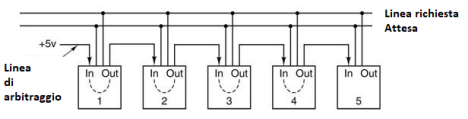
\includegraphics[width=0.8\linewidth]{arb_dec.png}
                        \label{fig:ar_dec}
                        \end{figure}    
                        
                \end{itemize}
                    
        \end{itemize}
    
\end{itemize}

\newpage

\subsection{Macchina di Harvard}

\textbf{Definizione} La macchina di Harvard è un altro modello di elaboratore nato basandosi sull'elaboratore \textit{Harvard Mark I}, a differenza del modello di Von Neumann prevede 2 memorie diverse per le istruzioni e i dati.

\begin{figure}[ht]
    \centering
    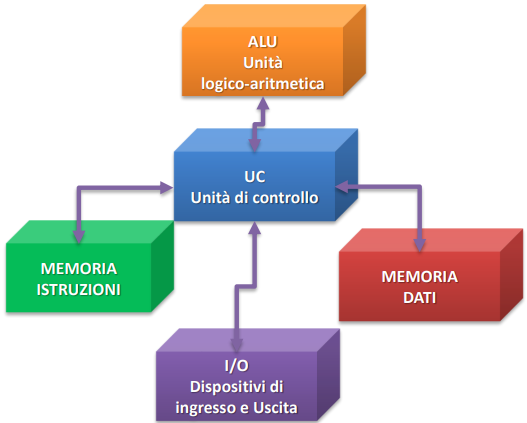
\includegraphics[width=0.7\linewidth]{harvard.png}
    \caption{Modello di Harvard}
    \label{fig:harvard}
\end{figure}

\section{Programmi}

L'esecuzione di un programma è l'ultimo passo di un processo che inizia con la scrittura dello stesso in un linguaggio simbolico di alto livello, le 3 entità che generalmente sono coinvolte in questo processo sono:
\begin{enumerate}
    \item \textbf{Compilatore}

        Trasforma il programma in linguaggio assembly, ottimizza il codice ed effettua un eventuale riordino delle istruzioni.
    
    \item \textbf{Assemblatore}

        Traduce il programma assembly in un file oggetto che è una combinazione di istruzioni macchina, dati ed altre informazioni.

        \newpage

        I file oggetto sono divisi solitamente in 6 sezioni:
        \begin{enumerate}
            \item \textbf{Object File Header}

                Contiene le locazioni e le dimensioni delle altre sezioni.

            \item \textbf{Text Segment}

                Contiene le istruzioni.

            \item \textbf{Data Segment}

                Contiene i dati.

            \item \textbf{Relocation information}

                Identifica istruzioni/dati che dovranno essere rilocati dal linker.

            \item \textbf{Symbol Table}

                Contiene i simboli non ancora definiti.

            \item \textbf{Debugging information}

                Contiene informazioni per il debug.
            
        \end{enumerate}

        Quando sono disposti in memoria è presente inoltre uno spazio apposito in cui si scambiano dati.
    
    \item \textbf{Linker}

        Il linker crea il file eseguibile partendo da quello oggetto, nel caso un programma ne abbia diversi allora essi vengono opportunamente collegati.\newline
    
\end{enumerate}

\noindent Una volta che il file eseguibile è pronto e si vuole eseguirlo entra in gioco il \textbf{Loader} che si occupa di caricarlo in memoria.\newline

\noindent Un'alternativa a questo processo è l'\textbf{interprete} che traduce direttamente le istruzioni senza bisogno di compilazione al costo di maggiore memoria e minore velocità di esecuzione.\newline

\subsection{Istruzioni}

\textbf{Definizione} Un'istruzione è una stringa binaria che indica all'elaboratore i compiti da svolgere, è divisa in sottostringhe definiti campi:
\begin{itemize}
    \item \textbf{OPCODE}

        Specifica il tipo di operazione.

    \item \textbf{Operando} 

        Può contenere un dato, un riferimento ad esso o l'etichetta di un registro.\newline
    
\end{itemize}

\newpage

\noindent Il tipo di suddivisione individua il formato dell'istruzione:
\begin{itemize}
    \item Lunghezza fissa

        Le istruzioni hanno una dimensione prefissata.

    \item Lunghezza variabile

        La dimensione cambia in base all'operazione.\newline
    
\end{itemize}

\noindent Quando si programma si utilizzano le istruzioni assembly che sono una rappresentazione simbolica delle istruzioni macchina, infatti tra le 2 esiste un legame uno a uno. In alcuni casi esistono delle pseudoistruzioni che sono composte da più istruzioni elementari. Generalmente sono costituite da:
\begin{itemize}
    \item L'indirizzo dell'istruzione in memoria
    \item Un'etichetta
    \item L'istruzione, comprende:
        \begin{itemize}
            \item Un codice mnemonico
            \item Il modo di indirizzamento
        \end{itemize}
    \item Eventuali commenti\newline
\end{itemize}

\noindent Esattamente come nei linguaggi di alto livello è possibile definire una \textbf{Macro} che permette di accorpare più istruzioni sotto un'etichetta, ovviamente quando si procede ad assemblare il programma sia queste che le pseudoistruzioni vengono sostituite.\newline

\noindent Prima di vedere le istruzioni generalmente presenti è opportuno definire le principali \textit{Flag} relative alla ALU:
\begin{itemize}
    \item \textbf{C} (Carry), 1 se l'ultima operazione ha prodotto un riporto/prestito
    \item \textbf{N} (Negative), 1 se l'ultima operazione ha prodotto un risultato negativo
    \item \textbf{Z} (Zero), 1 se l'ultima operazione è nulla
    \item \textbf{W} (Overflow), 1 se l'ultima operazione ha generato un Overflow
    \item \textbf{P} (Parity), 1 se l'ultima operazione ha dato un risultato con un numero pari di 1
\end{itemize}

\subsubsection{Classi}

Segue una carrellata di istruzioni generali:

\begin{table}[H]
\begin{adjustwidth}{-2.7cm}{}
    \centering
    \begin{tabular}{|c|c|l|}
    \hline
        Codice mnemonico & Operandi & \multicolumn{1}{c|}{Funzione} \\
    \hline
        \multicolumn{3}{|c|}{\textbf{Spostamento}}\\
    \hline
        LOAD & sorg,dest & Copia il valore della sorgente(memoria) nel destinatario \\
    \hline
        STORE & sorg,dest & Copia il valore della sorgente nel destinatario(cella di memoria esplicita) \\
    \hline
        MOVE & sorg,dest & Sposta il contenuto della sorgente nel destinatario (entrambi registri)\\
    \hline
        PUSH & sorg & Sposta il contenuto della sorgente in cima alla Stack \\
    \hline
        POP & dest & Sposta l'elemento in cima alla Stack nella destinazione \\
    \hline
        \multicolumn{3}{|c|}{\textbf{Aritmetiche}}\\
    \hline
        ADD & dest,sorg,sorg & Inserisce nella destinazione la somma dei valori delle sorgenti \\
    \hline
        CMP & dest,sorg,sorg & Inserisce nella destinazione la comparazione dei valori delle sorgenti \\
    \hline
        NEG & dest,sorg & Inserisce nella destinazione la negazione del valore della sorgente \\
    \hline
        \multicolumn{3}{|c|}{\textbf{Logiche}}\\
    \hline
        AND & dest,sorg,sorg & Inserisce nella destinazione l'AND dei valori delle sorgenti \\
    \hline
        OR & dest,sorg,sorg & Inserisce nella destinazione l'OR dei valori delle sorgenti \\
    \hline
        XOR & dest,sorg,sorg & Inserisce nella destinazione lo XOR dei valori delle sorgenti \\
    \hline
        NOT & dest,sorg & Inserisce nella destinazione il NOT del valore della sorgente \\
    \hline
        SL & reg,k & Shift a sinistra di k posti del registro \\
    \hline
        SR & reg,k & Shift a destra di k posti del registro \\
    \hline
        ROL & reg,k & Rotazione a sinistra di k posti del registro \\
    \hline
        ROR & reg,k & Rotazione a destra di k posti del registro \\
    \hline
        \multicolumn{3}{|c|}{\textbf{Implicite}}\\
    \hline
        CLRC & - & Imposta a 0 la flag C \\
    \hline
        CLRN & - & Imposta a 0 la flag N \\
    \hline
        CLRZ & - & Imposta a 0 la flag Z \\
    \hline
        CLRW & - & Imposta a 0 la flag W \\
    \hline
        SETC & - & Imposta a 1 la flag C \\
    \hline
        SETN & - & Imposta a 1 la flag N \\
    \hline
        SETZ & - & Imposta a 1 la flag Z \\
    \hline
        SETW & - & Imposta a 1 la flag W \\
    \hline
        \multicolumn{3}{|c|}{\textbf{Salto}}\\
    \hline
        BEQZ & sorg,ind & Se il valore della sorgente è 0 salta all'indirizzo \\
    \hline
        BGT & sorg1,sorg2,ind & Se sorg1$>$sorg2 salta all'indirizzo \\
    \hline
        BLT & sorg1,sorg2,ind & Se sorg1$<$sorg2 salta all'indirizzo \\
    \hline
        J & ind & Salta all'indirizzo \\
    \hline
        JSR & ind & Salva il valore di PC nella stack e salta all'indirizzo di subroutine \\
    \hline
        RET & - & Ripristina il valore di PC recuperandolo nella Stack\\
    \hline
        \multicolumn{3}{|c|}{\textbf{Comando}}\\
    \hline
        HALT & - & Interruzione di sistema\\
    \hline
        NOP & - & Nessuna operazione\\
    \hline
        BREAK & - & Interruzione di programma\\
    \hline
        
    \end{tabular}
\end{adjustwidth}
\label{tab:istr}
\end{table}

\subsubsection{Modi di indirizzamento}

Per poter esprimere dove risiede un operando esistono 2 modi:
\begin{enumerate}

    \item \textbf{Implicito}

        In alcune macchine gli operandi si trovano in posizioni prestabilite, non serve specificarli.

    \item \textbf{Assoluto} (Esplicito)

        Si indica il suo indirizzo.

\end{enumerate}

\vspace{5pt}

\noindent\textbf{Definizione} L'indirizzo effettivo è un indirizzo che prende 2 significati diversi in base al tipo di operazione:
\begin{enumerate}
    \item Nelle istruzioni logico-aritmetiche e di trasferimento dati è l'indirizzo degli operandi interessati
    \item In un'istruzione di salto è l'indirizzo dove si vuole andare.
\end{enumerate}

\vspace{5pt}

\noindent\textbf{Definizione} Un'etichetta è il designatore simbolico di un indirizzo in memoria.\newline

\noindent Esistono molti modi per indicare l'indirizzo di un operando: 
\begin{itemize}
    \item \textbf{Immediato}

        L'operando si trova nella posizione immediatamente successiva all'istruzione.

    \item \textbf{Diretto}

        Si usa l'indirizzo effettivo in memoria.   

    \item \textbf{A registro}

        Si usa l'etichetta del registro.

    \item \textbf{Indiretto}

        Si usa un indirizzo che punta ad un altro indirizzo.

    \item \textbf{Indiretto a registro}

        Come quello a registro ma esso contiene un indirizzo.

    \item \textbf{Indiretto differito}

        Come il precedente ma l'indirizzo punta ad un altro indirizzo.

    \item \textbf{Con spiazzamento}

        Come quello indiretto a registro ma ad esso si aggiunge un offset.

    \item \textbf{Relativo}

        L'indirizzo è dato dal PC ed un offset.

    \item \textbf{Pre/Post incremento/decremento}

        Come l'indiretto a registro ma il contenuto dello stesso viene incrementato/decrementato prima/dopo l'esecuzione dell'istruzione.
    
\end{itemize}

\subsection{Interruzioni}

\textbf{Definizione} Un'interruzione è un evento che cambia la normale sequenza di esecuzione di un programma, le possibili cause possono essere molteplici e non necessariamente dovute ad errori.\newline

\noindent Gli elaboratori possono avere 2 tipi di sistemi per gestire le eccezioni:
\begin{enumerate}
    \item \textbf{Mascherabile}

        Un'interruzione può essere interrotta da un'altra interruzione.
    
    \item \textbf{Non mascherabile}

        Un'interruzione deve essere gestita prima di gestirne un'altra.
    
\end{enumerate}

\vspace{7pt}

\noindent Quando si verifica un'interruzione il controllo viene passato ad un gestore che svolge le azioni appropriate e alla fine fa riprendere il programma dalla posizione in cui si trovava, questo sistema deve quindi garantire che:
\begin{itemize}
    \item Non ci siano interferenze sul processo interrotto, il contesto viene salvato

        Le fasi di commutazione del contesto sono protette, ossia non possono essere interrotte.
    
    \item Il dispositivo generatore venga individuato
    \item Multiple interruzioni vengano gestite secondo una priorità
\end{itemize}

\vspace{7pt}

\noindent L'uso di questo sistema implica che in memoria siano presenti tante routine di servizio (ISR) quanti sono i dispositivi e le possibili interruzioni software, queste richiedono che ci sia una corretta identificazione dei dispositivi. 

\subsubsection{Identificazione}

Ci sono 2 modi diversi per individuare le interruzioni:
\begin{enumerate}
    \item \textbf{Polling}

        Un dispositivo ha un registro che segnala se è presente un'interruzione, la CPU alla fine dell'esecuzione di un'operazione li controlla tutti, questo si può implementare tramite una porta OR o un collegamento \textit{wired OR} di porte open collector.

    \item \textbf{Int. vettorizzata}

        Una versione migliorata del Polling dove i dispositivi hanno un ulteriore registro che contiene un codice identificativo inviato al processore quando si verifica un'interruzione, questo valore solitamente punta all'inizio della routine necessaria.\newline 
        
\end{enumerate}

\noindent\textbf{Definizione} Il driver di una periferica è l'insieme di routine che servono per gestire le interazioni con esso.\newline

\subsubsection{Classificazione}

\noindent Esistono 2 principali metodi di classificazione, il primo in base all'origine:
\begin{itemize}
    \item Int. Hardware

        Proviene da un componente esterno.
    
    \item Int. Software

        Proviene dal programma stesso:
        \begin{enumerate}
            \item \textbf{Trap}

                Richiesta dal programmatore

            \item \textbf{Eccezione}

                Dovuta ad errori.\newline
            
        \end{enumerate}
    
\end{itemize}

\noindent Il secondo in base alla sua relazione con il clock:
\begin{itemize}
    \item Asincrone (Interne/Esterne)

        Potrebbero accadere in qualsiasi momento.
    
    \item Sincrone (Trap)

        Il loro accadimento è noto.\newline
    
\end{itemize}

\section{RISC/CISC e microprogrammazione}

\subsection{Microprogrammazione}

Alla fine degli anni cinquanta si dotò la CU di un decodificatore sequenziale e di una ROM in cui archiviare le sequenze dei comandi, l'idea era di far corrispondere un'istruzione all'esecuzione di un microprogramma scritto nella ROM.\newline

\noindent In questo caso il processore fa da interprete ad un linguaggio micro-programmato, la CU dovrà svolgere la seguente trasformazione:

$$\text{Micro-programma}\rightarrow\text{Insieme di micro-istruzioni}\rightarrow\text{Insieme di micro-operazioni}$$\newline

\newpage

\noindent I componenti essenziali di questa macchina sono:
\begin{itemize}
    \item Il generatore di indirizzo (della micro-istruzione)
    \item Il registro RAR (essenzialmente un program counter interno)\newline
\end{itemize}

\begin{figure}[ht]
    \centering
    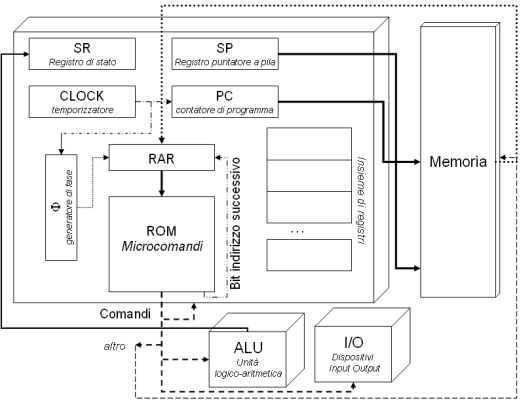
\includegraphics[width=0.9\linewidth]{micro.png}
    \label{fig:micro}
\end{figure}

\noindent Il micro-codice si può categorizzare in base alla sua struttura:
\begin{itemize}
    \item \textbf{Orizzontale}

        Si massimizzano la flessibilità e la parallelizzazione.

    \item \textbf{Verticale}

        Si privilegia la compattezza del codice.

    \item \textbf{Diagonale}

        Una combinazione delle precedenti.
    
\end{itemize}

\newpage

\subsection{CISC}
Le macchine CISC (Complex Instruction Set Computing) nacquero alla fine degli anni settanta, hanno un set di istruzioni complesse numeroso e spesso a lunghezza variabile.\newline

\noindent L'uso di istruzioni complesse era giustificato in quegli anni a causa della tecnologia disponibile:
\begin{itemize}
    \item Compilatori basilari 
    \item RAM costosa 
    \item No Cache
    \item Facile sostituzione della ROM contenente il set\newline
\end{itemize}

\noindent Ovviamente le istruzioni di questo tipo presentano degli svantaggi:
\begin{itemize}
    \item Molti cicli di clock per l'esecuzione
    \item Nel caso le operazioni non vengano scomposte serve una grande quantità di componenti per eseguirle
    \item Ogni istruzioni richiede accessi ed operazioni multiple, soprattutto nel giusto ordine
\end{itemize}

\subsection{RISC}

Le macchine RISC (Reduced Instruction Set Computer) nacquero nel 1980, questi nuovi processori avevano un set di istruzioni semplici e limitate in modo da poter sfruttare anche la pipeline.\newline


\begin{table}[H]
    \centering
    \begin{adjustwidth}{-4.25cm}{}
    \begin{tabular}{c|c|c|c|c|c|c|c}
         & Dimensione istr. & Formato istr. & Durata istr. & Complessità istr. & Num. registri & Modi ind. & Operazioni\\
         \hline
         \textbf{CISC} & Variabile & Variabile & Variabile & Complessa & Pochi & Complessi & Operandi in memoria\\
         \hline
         \textbf{RISC} & Fissa & Uniforme & Fissa & Semplice & Molti & Semplici & Op. ALU solo tra registri \\
    \end{tabular}
    \caption{Comparazione}
    \end{adjustwidth}
    \label{tab:cisc/risc}
\end{table}

\newpage

\section{Pipeline}

\textbf{Definizione} La canalizzazione è una tecnica che consiste nello scomporre una rete combinatoria inserendo dei registri di disaccoppiamento, questo permette di aumentare la frequenza del clock e svolgere più fasi in parallelo.\newline

\noindent In una macchina di tipo RISC ogni istruzione viene eseguita in 5 fasi:
\begin{enumerate}
    \item \textbf{Fetch}
    \item \textbf{Decode}
    \item \textbf{Execution}
    \item \textbf{Memory}
    \item \textbf{Write Back}
\end{enumerate}

\noindent Normalmente è attivo solo un "blocco" del circuito alla volta (associato ad una fase), invece tramite la pipeline ogni blocco elabora la fase di un'istruzione e passa subito alla successiva.\newline

\noindent Tutto questa risulta più arduo da implementare nel caso di macchine con istruzioni complesse e con tempi di esecuzione variabili, questo sia perché la frequenza del clock va regolata in modo da permettere l'esecuzione di ogni istruzione in parallelo sia perché alcune fasi potrebbero sovrapporsi tra di loro con istruzioni di lunghezza non fissa.\newline

\begin{figure}[ht]
    \centering
    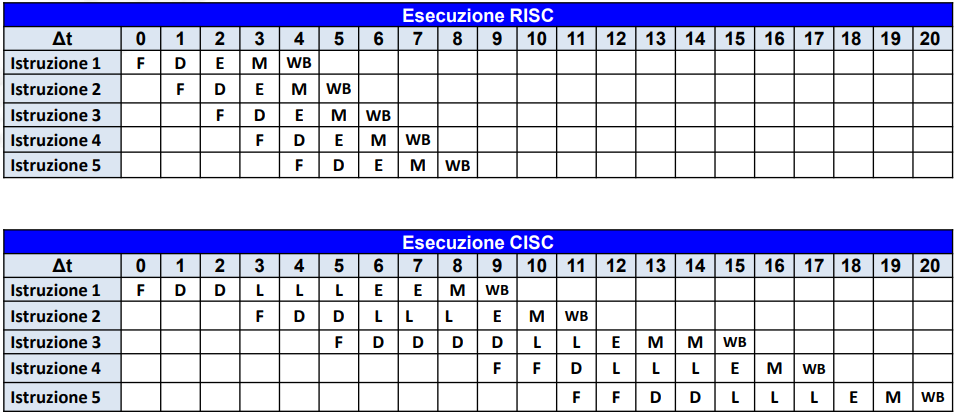
\includegraphics[width=\linewidth]{pipe.png}
    \caption{Esempio di esecuzione}
    \label{fig:pipe}
\end{figure}

\subsection{Hazard}

Ovviamente con questo sistema si potrebbero presentare dei problemi durante l'esecuzione (Hazard), si possono classificare in 3 categorie:
\begin{enumerate}
    \item \textbf{Sul controllo}

        Un salto o un'interruzione cambiano il flusso di esecuzione.
    
    \item \textbf{Sui dati}

        Un dato necessario sta venendo ancora usato in un'istruzione precedente.

    \item \textbf{Strutturali}

        Non sono sufficienti le risorse Hardware.\newline
    
\end{enumerate}

\noindent Per cercare di risolvere il problema si possono utilizzare diversi metodi:
\begin{itemize}
    \item \textbf{Forwarding}

        Se il dato serve nell'istruzione successiva si può inserire una scorciatoia che permetta di passare il dato prima della fase WB.

    \item \textbf{Stallo}

        In caso non sia possiibile usare il Forwarding si inseriscono degli stalli che ritardano l'esecuzione di qualche ciclo.

    \item \textbf{Riordino}

        Viene cambiata la sequenza delle istruzioni per evitare gli stalli, bisogna però mantenere la semantica.

    \item \textbf{Anticipo}

        I salti incondizionati si possono riconoscere in una fase precedente risparmiando un'istruzione. 

    \item \textbf{Branch Prediction}

        La CPU osserva i salti e cerca di pre-caricare l'istruzione da eseguire.
    
\end{itemize}

\newpage

\section{DMA}

La soluzione migliore per interfacciarsi con dispositivi I/O è l'accesso diretto alla memoria, tramite un apposito controllore è possibile trasferire dati da/a il dispositivo senza dover passare ogni volta per il processore.\newline

\noindent Questo controllore contiene:
\begin{itemize}
    \item Il registro \textbf{CAR} (Current Address Register)

        Funge da puntatore alla locazione di memoria.

    \item Il \textbf{WC} (Word Counter)

        Contiene la quantità di dati da trasferire.

    \item Un registro di stato

    \item Delle linee di comando per gestire il trasferimento dei dati\newline
    
\end{itemize}

\begin{figure}[ht]
    \centering
    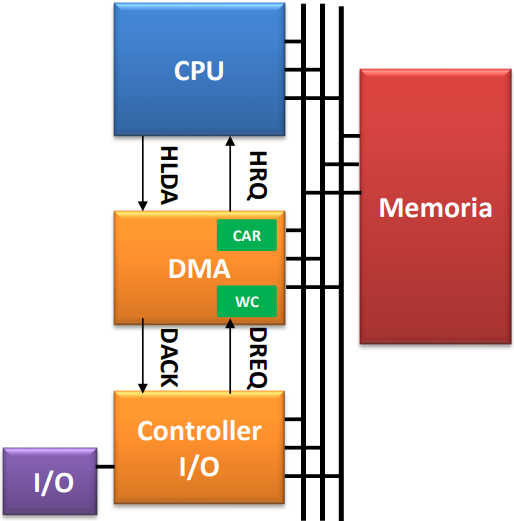
\includegraphics[width=0.65\linewidth]{DMA.png}
    \label{fig:dma}
\end{figure}

\noindent Per trasferire dei dati si segue il seguente procedimento:
\begin{enumerate}
    \item Si accede alla locazione di memoria 
    \item Si trasferisce una parola tramite il Bus
    \item Si incrementa/decrementa il CAR
    \item Si decrementa il WC
    \item Quando WC$=0$ crea un interruzione per segnalare la fine del trasferimento
\end{enumerate}

\section{Memorie}

A causa del costo e delle diverse prestazioni si stabilisce una gerarchia tra le diverse memorie usate in un elaboratore:
\begin{enumerate}
    \item \textbf{Registri}
    \item \textbf{Cache}
    \item \textbf{RAM}
    \item \textbf{Memorie non volatili}\newline
\end{enumerate}

\noindent Questa organizzazione a livelli permette ad un programmatore di avere una memoria che sia veloce e capiente contemporaneamente.\newline

\subsection{RAM}

La RAM è il tipo di memoria più usata come memoria centrale, ne esistono 2 tipi:


\begin{table}[ht]
    \centering
    \begin{tabular}{c|c}
          \textbf{SRAM} & \textbf{DRAM}\\
          \hline
          Accesso rapido & Accesso più lento\\
          \hline
          Costo alto & Costo minore\\
          \hline
          Maggiore consumo elettrico & Minore consumo elettrico\\
          \hline
          Circuiti complessi & Circuiti semplici\\
          \hline
          Bassa densità delle celle & Alta densità delle celle\\
    \end{tabular}
    \caption{Confronto tra RAM}
    \label{tab:ram}
\end{table}

\subsection{Cache}

L'inserimento di questa memoria si basa sul principio di località:
\begin{itemize}
    \item Località \textbf{temporale}

        Quando si usa un elemento in memoria molto spesso viene riutilizzato a breve.

    \item Località \textbf{spaziale}

        Quando si usa un elemento in memoria molto spesso vengono usati gli elementi ad esso vicini.\newline
    
\end{itemize}

\newpage

\noindent Fisicamente è organizzata in linee:

\begin{table}[ht]
    \centering
    \begin{tabular}{|c|c|c|}
        \multicolumn{1}{c}{V} & \multicolumn{1}{c}{TAG} & \multicolumn{1}{c}{DATA}\\
        \hline
         &  &\\
        \hline
         &  &\\
        \hline
         &  &\\
        \hline
         &  &\\
        \hline
         &  &\\
        \hline
    \end{tabular}
    \label{tab:cache}
\end{table}

I campi presenti sono:
\begin{itemize}
    \item \textbf{V}

        Indica se la linea contiene dei dati.
    
    \item \textbf{TAG}

        Identifica quale parola della memoria centrale è nella linea.
    
    \item \textbf{DATA}

        La parola effettiva.
    
\end{itemize}

\noindent Quando il processore richiede un certo dato viene controllata la Cache prima della memoria centrale, se non presente il valore viene anche caricato nella Cache e questo permette di diminuire il tempo medio per trovare un dato.\newline

\noindent Quando un dato nella Cache viene modificato bisogna aggiornare la memoria di livello inferiore, ci sono 2 modi:
\begin{itemize}
    \item \textbf{Write Through}

        Il blocco in memoria viene aggiornato ad ogni modifica.

    \item \textbf{Write Back}

        Il blocco in memoria viene aggiornato solo quando viene sostituito.\newline 
    
\end{itemize}

\newpage

\subsubsection{Tipi}

Esistono diversi tipi di Cache, la differenza sta nel come fanno corrispondere un indirizzo locale con uno della memoria centrale:
\begin{itemize}
    \item \textbf{Direct Mapped}

        $$\text{Ind. parola in Cache }=\text{ Ind. parola in memoria}\mod{\text{(Num. linee Cache)}}$$

    \item \textbf{Associativa a n-vie}

        Vengono definiti un certo numero $x$ di insiemi di $n$ parole, per trovare l'insieme in cui si trova una parola:

        $$\text{Insieme }=\text{ Ind. parola in memoria}\mod{x}$$

    \item \textbf{Completamente associativa}

        Una parola può essere inserita in qualsiasi posizione.\newline
        
\end{itemize}

\subsubsection{Politiche di rimpiazzo}

Quando si verifica un MISS e la Cache è piena bisogna stabilire (tranne nella Direct Mapped) quale degli elementi presenti può essere sostituito con il nuovo:
\begin{itemize}
    \item \textbf{Sostituzione casuale}
    \item \textbf{LRU} (Least Recently Used)

        Si usa un opportuno contatore che tiene traccia del tempo che un elemento passa nella Cache, si rimuove quello più "vecchio".
    
    \item \textbf{LFU} (Least Frequently Used)

        Si usa un opportuno contatore che tiene traccia di quante volte un elemento è stato usato, quello usato meno frequentemente viene rimosso.\newline
    
\end{itemize}

\newpage

\subsection{Allocazione dei processi}

\textbf{Definizione} Un processo è un programma presente in memoria centrale e che è in corso di esecuzione.\newline

\noindent Ogni processo ha un \textbf{PCB} (Process Control Block) associato che contiene:
\begin{itemize}
    \item Lo stato del processo
    \item Il suo program counter
    \item I valori nei registri
    \item Informazioni sullo scheduling
    \item Informazioni sulla memoria
    \item Informazioni di contabilità
    \item Informazioni I/O\newline
\end{itemize}

\noindent Considerando la quantità di processi normalmente attivi c'è necessità di allocare la memoria in modo efficiente, ci sono svariati metodi:
\begin{itemize}
    \item A partizione \textbf{singola}
    
        Ci può essere un solo processo allocato alla volta.

    \item A partizioni \textbf{multiple}
        \begin{itemize}
            \item A dimensione \textbf{fissa}

                Quando un programma deve essere caricato si crea una partizione.

            \item A dimensione \textbf{variabile}

                Una partizione viene allocata dinamicamente in base al processo.
            
        \end{itemize}

        In entrambi i casi è presente un problema definito frammentazione (risolvibile tramite la compattazione):
        \begin{itemize}
            \item \textbf{Interna}

                Viene allocata della memoria eccessiva per ogni processo e in presenza di molti diventa uno spreco importante di memoria.
    
            \item \textbf{Esterna}

                C'è abbastanza memoria per un processo ma non è contigua.\newline
            
        \end{itemize}
        
\end{itemize}

\noindent Nel caso un programma richieda più memoria della massima partizione possibile si può ricorrere all'\textit{Overlay}, esso permette di caricare in memoria solamente la parte di programma attualmente usata e scambiarla con opportune operazioni quando necessario (poco efficiente a causa degli scambi).\newline

\subsubsection{Memoria virtuale}

\textbf{Definizione} La memoria virtuale è una tecnica che consente di eseguire programmi anche se non possono essere contenuti pienamente della memoria.\newline

\noindent Per funzionare usa una tecnica chiamata \textit{Paginazione} che permette ad un programma di avere uno spazio degli indirizzi non per forza contiguo, funziona dividendo la memoria in "frame" ed il programma in "pagine" e caricando poi quest'ultime nei frame quando necessario.\newline

\noindent Facendo così si ottiene uno spazio di indirizzi logici, essi sono tradotti in indirizzi fisici usando la tabella delle pagine:

\begin{figure}[ht]
    \centering
    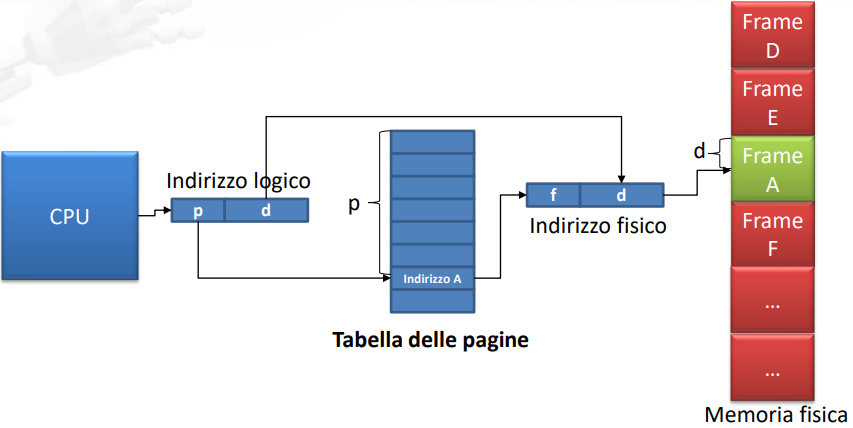
\includegraphics[width=\linewidth]{page.png}
    \caption{Traduzione degli indirizzi}
    \label{fig:virt_page}
\end{figure}

\newpage

\noindent Un esempio di funzionamento è il seguente:
\begin{enumerate}
    \item Il processore richiede un indirizzo logico
    \item Viene cercata la pagina nella tabella
    \item Non è presente, si genera un'interruzione
    \item Controllando il PCB si cerca l'indirizzo, se è valido passa al punto successivo
    \item Si cerca un frame libero
    \item Viene caricata la pagina in quel frame tramite I/O e si aggiornano le tabelle
    \item L'istruzione viene riavviata
\end{enumerate}

\begin{figure}[ht]
    \centering
    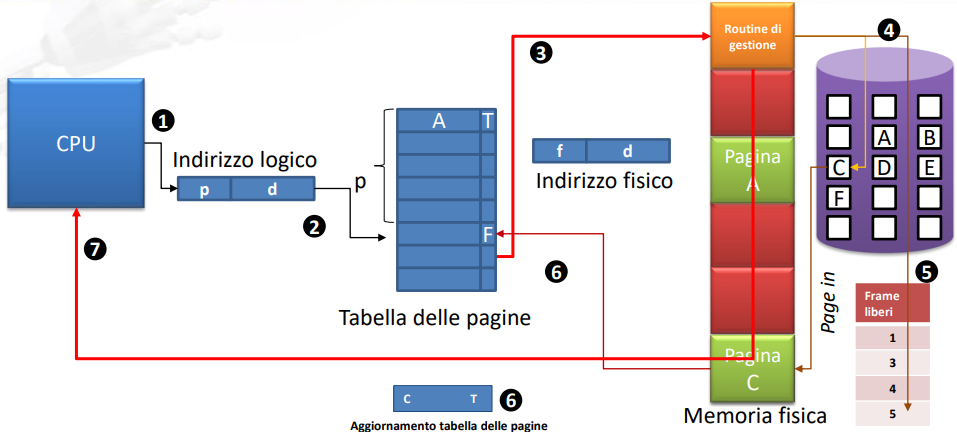
\includegraphics[width=\linewidth]{virt.png}
    \caption{Rappresentazione grafica}
    \label{fig:virt}
\end{figure}

\noindent Come si è visto se una pagina non è presente in memoria va caricata dalla memoria secondaria (On-Demand Paging), in alternativa è possibile usare il \textit{Prepaging} che consiste nel caricare a "blocchi" le pagine contigue.\newline

\newpage

\noindent Nel caso ci sia bisogno di inserire una pagina nella memoria piena si adottano diversi metodi per scegliere il rimpiazzo:
\begin{itemize}
    \item \textbf{LRU} (Come per la Cache)

    \item \textbf{FIFO}

        Si scambia con la pagina presente in memoria da più tempo.

    \item \textbf{CLOCK}

        Le pagine vengono organizzate in una coda circolare insieme ad un bit che indica se sono state usate, quando bisogna scambiare si ispeziona tutta la coda e:
        \begin{itemize}
            \item Se il bit è 1 viene settato a 0
            \item Se il bit è 0 viene sostituita la pagina
        \end{itemize}

    \item \textbf{OPT} (Soluzione ottimale utopistica)
    
\end{itemize}

\section{Sistemi operativi (Fondamenti)}

\textbf{Definizione} Il Firmware è un programma eseguibile che sia avvia automaticamente dopo l'accensione della macchina, tipicamente risiede su una EEPROM.\newline

\noindent I principali compiti che svolge sono:
\begin{enumerate}
    \item Controllare il funzionamento dei vari componenti
    \item Eseguire il \textit{Bootloader}, ossia caricare in memoria il Kernel (Nucleo) del Sistema Operativo\newline
\end{enumerate}

\begin{figure}[ht]
    \centering
    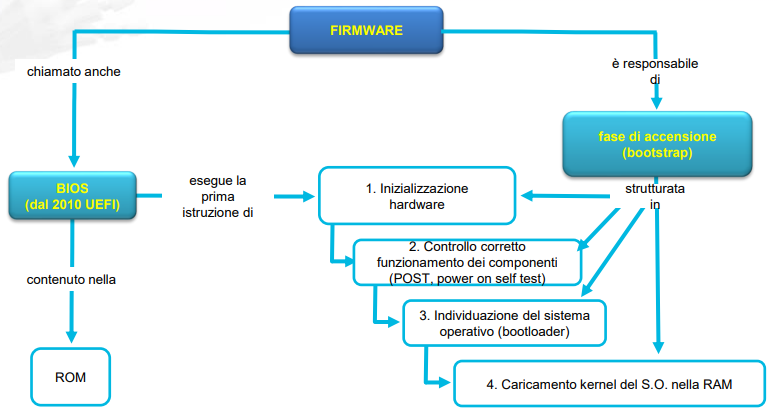
\includegraphics[width=0.85\linewidth]{firm.png}
    \label{fig:firmware}
\end{figure}

\noindent Una volta caricato il S.O. rimane sempre in esecuzione ed il suo Kernel è sempre in memoria centrale.\newline

\noindent\textbf{Definizione} Il sistema operativo è un insieme di programmi che:
\begin{itemize}
    \item Gestisce le componenti fisiche dell'elaboratore
    
    \item Fornisce un ambiente in cui è possibile installare, gestire ed eseguire i programmi applicativi

    \item Permette l’interazione utente-elaboratore senza che esso conosca tutti i dettagli dell’architettura

\end{itemize}

\begin{figure}[ht]
    \centering
    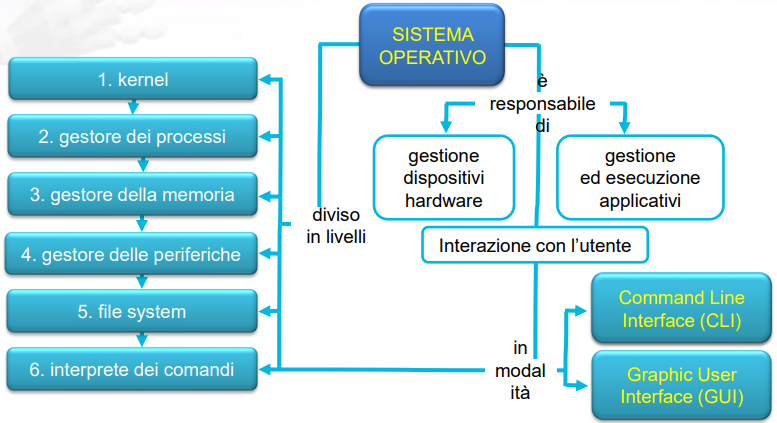
\includegraphics[width=0.8\linewidth]{so.png}
    \label{fig:so}
\end{figure}

\noindent Essenzialmente deve gestire interamente la macchina svolgendo tutti i compiti:

\begin{figure}[ht]
    \centering
    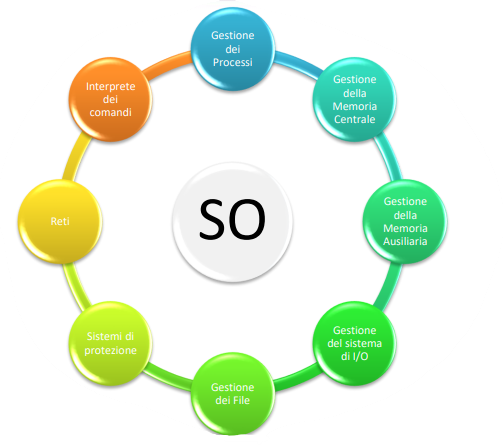
\includegraphics[width=0.6\linewidth]{so2.png}
    \caption{Compiti principali}
    \label{fig:so2}
\end{figure}

\section{Architetture Multiprocessore e multicore}

\textbf{Definizione} I sistemi multiprocessore e multicore sono rispettivamente definiti come:
\begin{itemize}
    \item "Sistema con 2 o più processori operanti in parallelo"
    \item "Sistema composto da 2 o più core (nucleo del processore) nello stesso chip"\newline
\end{itemize}

\noindent Entrambe sono architetture che permettono il calcolo parallelo, risulta utile dare una classificazione delle architetture viste fin'ora tramite la tassonomia di Flynn:

\begin{figure}[ht]
    \centering
    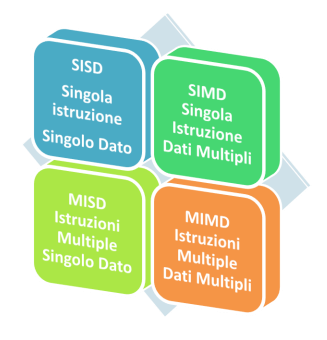
\includegraphics[width=0.5\linewidth]{flynn.png}
    \label{fig:flynn}
\end{figure}

\begin{itemize}
    \item \textbf{SISD}

        Quella classica, un solo processore.

    \item \textbf{MISD} (Instruction Level Parallelism)

        Sono presenti più processori che svolgono un istruzione ciascuno contemporaneamente sullo stesso dato.

    \item \textbf{SIMD} (Data Level Parallelism)

        Contiene più processori tra cui si individua quello "Master", esso rilascia un flusso di istruzioni che vengono eseguite una alla volta da ogni processore su dati diversi. 

    \item \textbf{MIMD} (Thread Level Parallelism)

        Ogni processore è autonomo, ha la propria CU e la sua memoria locale.\newline
    
\end{itemize}

\subsection{Gestione della memoria}

Nel caso multiprocessore è possibile avere una memoria:
\begin{itemize}
    \item \textbf{Condivisa}
        \begin{itemize}
            \item La memoria è la stessa per tutti i processori
            \item Può accedere un solo processore alla volta
            \item Eventuali zone comuni vanno gestite dal programmatore
        \end{itemize}

        Ce ne sono 2 tipi:
        \begin{itemize}
            \item \textbf{Uniform Memory Acess}

            \item \textbf{Non Uniform Memory Acess}

                La memoria viene divisa in zona comune e zona veloce.
                
        \end{itemize}
    
    \item \textbf{Distribuita}
        \begin{itemize}
            \item La memoria è distribuita fisicamente tra i processori
            \item Per comunicare tra loro i processori usano il \textit{Message Passing}
        \end{itemize}

        Ce ne sono 2 tipi:
        \begin{itemize}
            \item  \textbf{NO-Remote Memory Access}

                Tutte le memorie locali sono private.

            \item \textbf{Cache Only Memory Access}

                Presenti solo le memorie Cache.
                
        \end{itemize}
    
\end{itemize}

\subsection{Gestione dei processi}

\textbf{Definizione} Un thread è una suddivisione di un processo in 2 o più sottoprocessi.\newline

\noindent\textbf{Definizione} Il multithreading è la capacità di un processore di passare da un thread all'altro.\newline

\noindent I 3 tipi principali di Multithreading sono:
\begin{enumerate}
    \item \textbf{Coars Grained MultiThreading}

        Si esegue un thread alla volta, appena si presenta uno stallo prolungato si passa ad un altro.

    \item \textbf{Fine Grained MultiThreading}

        Ad ogni ciclo di clock vengono alternati i thread.

    \item \textbf{Simultaneous MultiThreading}

        Una combinazione dei precedenti.
    
\end{enumerate}

\section{Memorie di massa}

Le memorie di massa sono classificabili in base al tipo di accesso:
\begin{itemize}
    \item \textbf{Sequenziale}
    \item \textbf{Diretto}
    \item \textbf{Indicizzato}
\end{itemize}

\noindent E al loro materiale di composizione:
\begin{itemize}
    \item \textbf{Magnetico}
    \item \textbf{Ottico}
    \item \textbf{A stato solido}\newline
\end{itemize}

\noindent\textbf{Definizione} Un documento digitale è una collezione di dati organizzata secondo un certo formato.\newline

\noindent\textbf{Definizione} Un supporto digitale è una memoria su cui viene archiviato un documento digitale.\newline

\noindent\textbf{Definizione} Un oggetto digitale è un supporto digitale contenente un documento digitale ed una sua descrizione.\newline

\subsection{Nastro magnetico}

Il nastro magnetico è formato da uno strato di particelle magnetiche depositate su un supporto flessibile.\newline

\noindent I componenti principali sono:
\begin{itemize}
    \item \textbf{Rivestimento dorsale}
    \item \textbf{Substrato}
    \item \textbf{Strato magnetico}
    \item \textbf{Legante}\newline
\end{itemize}

\newpage

\noindent Ogni particella ha un verso di magnetizzazione, un insieme di particelle può mutare il suo verso in presenza di un campo magnetico esterno. La scrittura quindi avviene sfruttando un elettromagnete per cambiare l'orientamento, la lettura invece leggendo le variazioni del campo magnetico.\newline

\begin{figure}[ht]
    \centering
    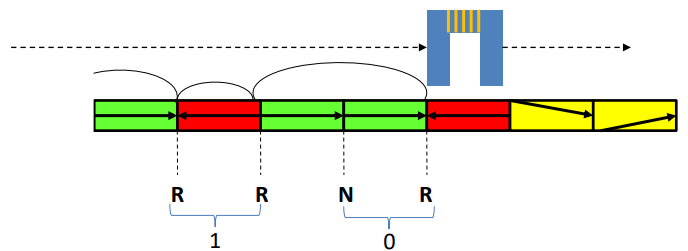
\includegraphics[width=0.7\linewidth]{nastro2.png}
    \label{fig:nastro_r}
\end{figure}

\noindent Il nastro viene diviso in tracce e a loro volta in blocchi, un blocco odierno è formato da:
\begin{enumerate}
    \item Preambolo
    \item Marcatore di inizio
    \item Sezione dati
    \item Indirizzo del blocco
    \item Informazioni per il rilevamento e la correzione di errori
\end{enumerate}

\begin{figure}[ht]
    \centering
    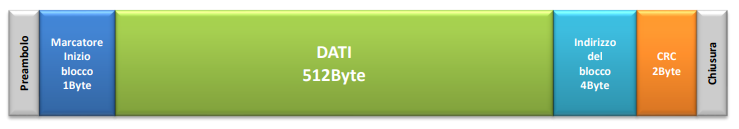
\includegraphics[width=0.7\linewidth]{nastro.png}
    \caption{Blocco LTO}
    \label{fig:blocco}
\end{figure}

\noindent I principali tipi sono:
\begin{itemize}
    \item Super Digital Linear Tape
    \item Super Advanced Intelligent Tape
    \item Linear Tape Open (STANDARD)
\end{itemize}

\newpage

\subsection{Disco magnetico}

Il disco magnetico è formato da uno strato di particelle magnetiche depositate su un supporto fisso.\newline

\noindent I componenti principali sono:
\begin{itemize}
    \item \textbf{Substrato}
    \item \textbf{Strato magnetico}
\end{itemize}

\vspace{5pt}

\noindent 2-3 dischi magnetici, il sistema di movimentazione e le testine sono sigillati in una custodia metallica a tenuta stagna chiamata Hard-Disk:

\begin{figure}[ht]
    \centering
    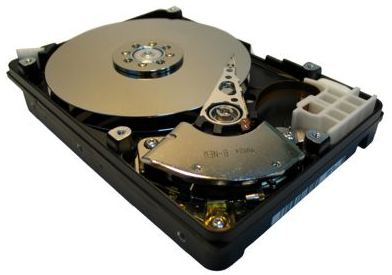
\includegraphics[width=0.3\linewidth]{harddisk2.png}
    \caption{Hard-Disk}
    \label{fig:harddisk2}
\end{figure}

\noindent Il funzionamento è simile al nastro magnetico.\newline

\noindent Il disco ha 2 facce, una faccia viene divisa in tracce e a loro volta in settori, più settori contigui formano un cluster. La quantità di dati nel settore può essere variabile o costante (nelle parti esterne ce ne sono di più).\newline

\noindent Una traccia è formata da:
\begin{enumerate}
    \item Preambolo
    \item Sincronizzazione
    \item Indirizzo del blocco
    \item Sezione dati
    \item Informazioni per il rilevamento e la correzione di errori
\end{enumerate}

\begin{figure}[ht]
    \centering
    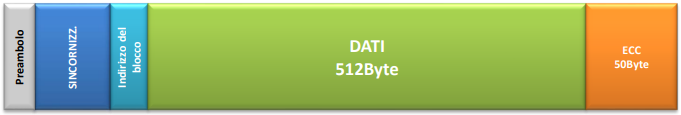
\includegraphics[width=0.65\linewidth]{harddisk.png}
    \caption{Blocco}
    \label{fig:harddisk}
\end{figure}

\subsection{Disco ottico}

Il disco ottico ha una struttura composta da materiali eterogenei.

\vspace{5pt}

\noindent I componenti principali sono:
\begin{itemize}
    \item \textbf{Substrato}
    \item \textbf{Strato dati}
    \item \textbf{Strato riflettente}
    \item \textbf{Strato protettivo}\newline
\end{itemize}

\begin{figure}[ht]
    \centering
    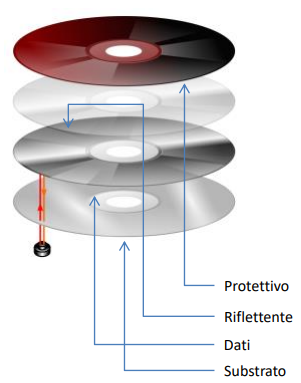
\includegraphics[width=0.4\linewidth]{cd.png}
    \caption{Struttura}
    \label{fig:cd}
\end{figure}

\noindent I dati vengono rappresentati da depressioni (pit) e spianate (land) sulla superficie e sono disposti a spirale, essa viene divisa in settori. Essendo nati per conservare la musica sono strutturati in modo da avere una densità dei dati costante che permette una velocità di lettura lineare costante.

\begin{figure}[ht]
    \centering
    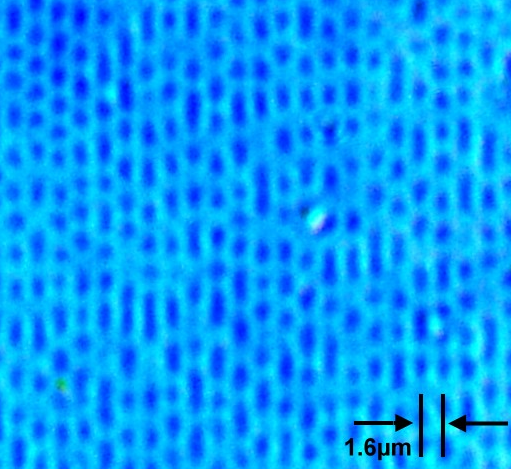
\includegraphics[width=0.3\linewidth]{cd2.png}
    \label{fig:cd2}
    \caption{Superfice al microscopio}
\end{figure}

\newpage

\noindent Per essere letti e scritti viene usato un laser che seguendo la traccia viene riflesso in modo variabile a causa della superficie e letto da un fotodiodo:
\begin{itemize}
    \item La transizione da pit a land (o viceversa) indica un 1
    \item Le parti "piatte" indicano una serie di 0
\end{itemize}

\begin{figure}[ht]
    \centering
    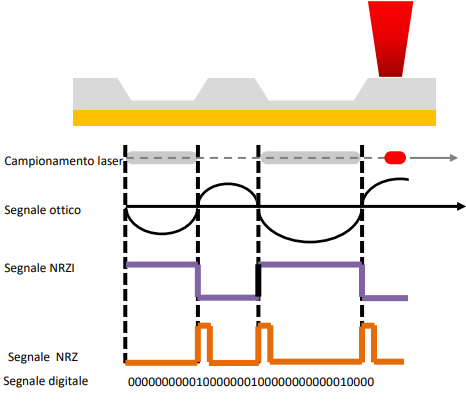
\includegraphics[width=0.7\linewidth]{disk.png}
    \caption{Lettura}
    \label{fig:disk}
\end{figure}

\noindent La scrittura varia in base al tipo di disco, partendo da un file ISO:
\begin{itemize}
    \item \textbf{Sola lettura} (CD-ROM,DVD-ROM,BR-ROM)
    
        Si imprimono i pit su un disco master (in vetro o 
        zinco) e poi si effettua uno stampo versando la base in 
        policarbonato allo stato fuso.

    \item \textbf{Registrabili una volta} (CD-R,DVD-R,BR-R)

         Si brucia una pellicola organica grazie al masterizzatore, la fusione della pellicola (che copre lo strato riflettente) produce delle aree riflettenti che vanno a ripetere la condizione di opacità e riflettività dei pit e dei land.

        \item \textbf{Riscrivibili} (CD-RW,DVD-RW,BR-RW)

        Si usa del materiale cristallino, quando il laser è alla massima potenza il materiale si scoglie creando una zona amorfa e perdendo di riflettività, questa differenza con il materiale "normale" va a simulare i pit e i land. 
        
        
        Per farlo ritornare vuoto basta scaldare le zone amorfe a circa 200°C, questo fa ritornare la riflettività del materiale.\newline
    
\end{itemize}

\noindent Inserendo una tabella dei contenuti nella parte centrale è possibile migliorare la ricerca dei file sul disco indicandone la posizione.\newline

\noindent Una particolarità è l'uso della modulazione Eight-to-fourteen (nei CD), la sua caratteristica è il trasformare un byte in una parola di 14 bit avente gli 1 separati da 2-10 0.\newline

\noindent I principali tipi sono:
\begin{itemize}
    \item \textbf{CD}
    \item \textbf{DVD}
    \item \textbf{Blu-ray}
    \item \textbf{HVD}
\end{itemize}

\noindent Ogni tipo usa laser e lenti diverse:

\begin{figure}[ht]
    \centering
    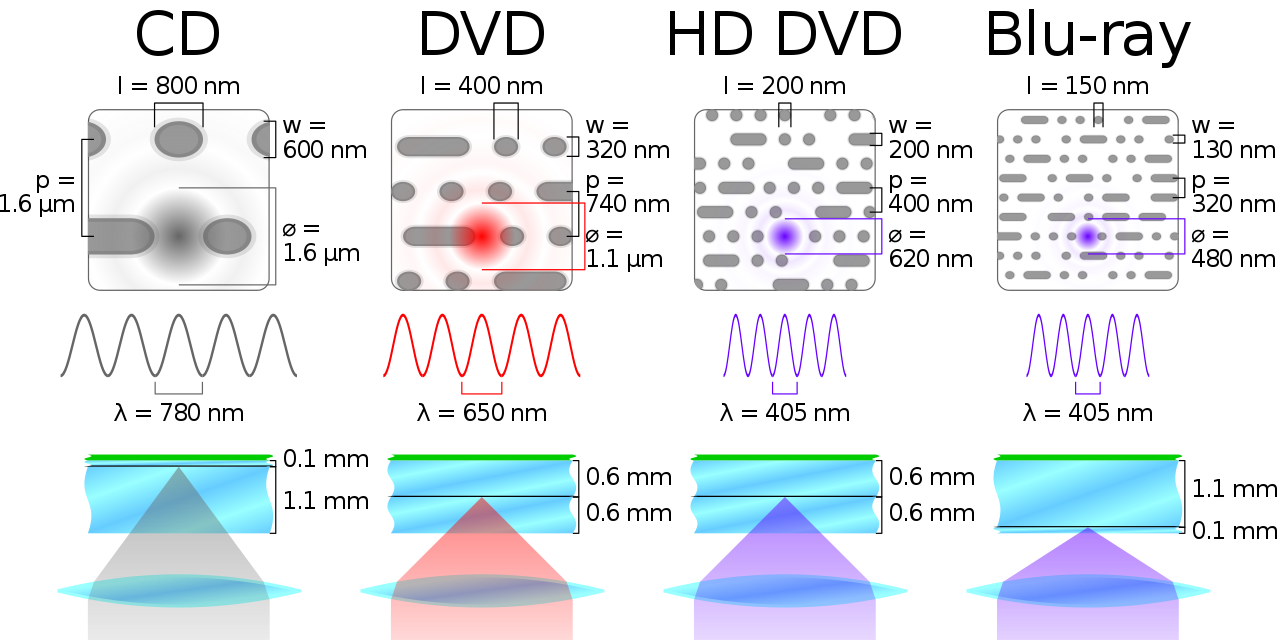
\includegraphics[width=\linewidth]{Comparison_CD_DVD_HDDVD_BD.svg.png}
    \label{fig:cd3}
\end{figure}

\newpage

\subsection{A stato solido}

Le memorie a stato solido sono delle matrici di celle di memoria, nella maggior parte si usa un transistor a griglia fluttuante per mantenere l'informazione:

\begin{figure}[ht]
    \centering
    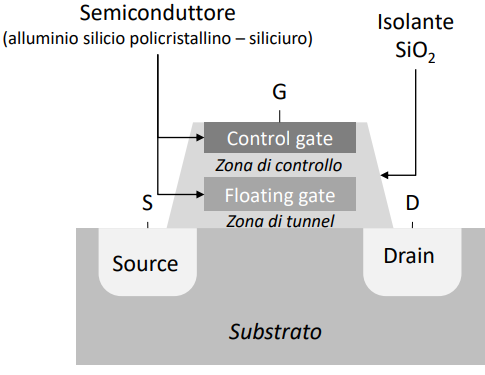
\includegraphics[width=0.7\linewidth]{trans.png}
    \label{fig:transistor}
\end{figure}

\noindent Per scrivere si applicano 7V al Drain e 12V al Control Gate, per cancellare invece 9V al Gate e 6V alla Source.\newline

\noindent Per leggere si applica 1V al Drain e se è presente un flusso di elettroni allora vale 1.\newline

\noindent Le celle si raggruppano in chunk, i chunk in pagine e le pagine in blocchi, i dati vengono recuperati con accesso casuale.\newline

\noindent Data la struttura la scrittura/modifica/cancellazione può avvenire solamente a blocchi, se una pagina deve essere cancellata sarà solamente contrassegnata come non valida. Questo porta inevitabilmente alla frammentazione interna, per ovviare al problema la memoria svolge periodicamente dei controlli tramite \textit{Garbage Collection}.\newline

\noindent Ogni volta che una cella viene scritta/cancellata la sua zona di tunnel si degrada, per migliorare l'aspettativa di vita della memoria si usa l'\textit{Overprovisioning} mantenendo uno spazio non allocato, in questo modo si riesce a garantire un numero di celle sostituibili adeguato.\newline

\newpage

\subsection{Digital Preservation}

\noindent\textbf{Definizione} La preservazione digitale è l'insieme di attività volte a garantire la durata nel tempo e la conservazione delle informazioni in formato digitale.\newline

\noindent Ogni tipo di memoria di massa può essere adatta o meno per preservare i dati nel lungo periodo:


\begin{table}[H]
    \centering
    \begin{adjustwidth}{-3.5cm}{}
    \begin{tabular}{c|c|c|c|c}
        Supporto & Aspettativa di vita & Capacità di archiviazione & Affidabilità progettuale & Obsolescenza tecnologica\\
        \hline
        Nastro magnetico & Lunga & Grande & Elevata & Bassa \\
        \hline
        Disco magnetico & Medio-bassa & Grande & Medio-bassa & Medio-elevata \\
        \hline
        Disco ottico & Medio-bassa & Media & Inesistente & Alta \\
        \hline
        Mem. stato solido & Bassa & Medio-alta & Scarsa & Bassa \\
    \end{tabular}
    \end{adjustwidth}
    \label{tab:dp}
\end{table}

\end{document}
